\documentclass[czech,master,public,dept470,male,cpdeclaration,oneside, python]{diploma}

\usepackage{subfig}		% makra pro "podobrazky" a "podtabulky"
\usepackage{tikz}		% makra pro kresleni

\usepackage{amsmath}
\usepackage{amssymb}

\usepackage{graphicx}
\usepackage{float} 
\usepackage{pgfplots} 
\graphicspath{  }
\usepackage{listings}
\usepackage{xspace}
\usepackage{color} %red, green, blue, yellow, cyan, magenta, black, white
\definecolor{mygreen}{RGB}{28,172,0} % color values Red, Green, Blue
\definecolor{mylilas}{RGB}{170,55,241}


\usepackage{xcolor}
%\newcommand\myworries[1]{\textcolor{red}{#1}}

\CzechAbstract{Práce se zabývá modelem po částech linearní regrese. Obsahuje stručný úvod do Bayesovské statistiky, pomcí níž zavádíme model pro po částech lineární regresi. Protože se s aposteriorním rozdělením dáneho modelu nedá analyticky pracovat, používáme pro jeho aproximaci algoritmus RJMCMC. K tomu se postupně dostáváme přes klasické MCMC metody. Na závěr práce prezentujeme výsledky dosažené za pomocí algoritmu RJMCMC, jehož implementace je součásti této práce a byla provedena v programovacím jazyce Python.}

\CzechKeywords{diplomová práce, Python, MCMC, RJMCM, Po částech lineární regrese, lineární regrese, Bayesovská statistika, Theano, SciPy}

\EnglishAbstract{This work is about segmented linear regression. It contains a brief introduction to Bayesian statistics, which we use to define a model for segmented linear regression. Posterior distribution for the model doesn't have a closed form, so we use RJMCMC algorithm to aproximate the distribution. Before introducing RJMCMC we give an overview of classical MCMC algorithms. At the end of the thesis we show examples of how RJMCMC works. We implemented the RJMCMC algorithm as part of the thesis, for that we used the programming language Python. }

\EnglishKeywords{master's thesis, Python, MCMC, RJMCMC, Piecewise linear regression, Segmented regression, Bayesian statistics, Theano, Scipy}


\lstset{language=python,%
    %basicstyle=\color{red},
    breaklines=true,%
    morekeywords={matlab2tikz},
    keywordstyle=\color{blue},%
    morekeywords=[2]{1}, keywordstyle=[2]{\color{black}},
    identifierstyle=\color{black},%
    stringstyle=\color{mylilas},
    commentstyle=\color{mygreen},%
    showstringspaces=false,%without this there will be a symbol in the places where there is a space
    numbers=left,%
    numberstyle={\tiny \color{black}},% size of the numbers
    numbersep=9pt, % this defines how far the numbers are from the text
    emph=[1]{for,end,break},emphstyle=[1]\color{red}, %some words to emphasise
    %emph=[2]{word1,word2}, emphstyle=[2]{style},    
}


% Dalsi doplnujici baliky maker
\usepackage{subfig}		% makra pro "podobrazky" a "podtabulky"
\usepackage{tikz}		% makra pro kresleni


% Zadame pozadovane vstupy pro generovani titulnich stran.
\ThesisAuthor{Martin Koběrský}

\CzechThesisTitle{Po částech lineární regrese}

\EnglishThesisTitle{Segmented Regression}

\SubmissionDate{13. července 2018}

% Pokud nechceme nikomu dekovat makro zapoznamkujeme.
\Thanks{Rád bych poděkoval panu Kracíkovi za shovívavost a trpělivost a svojí mamince za zkontrolování gramtických chyb. Pokud i přesto nějaké chyby zůstaly, chyba je jen na mojí straně. Děkuji.}

% Zadame cestu a jmeno souboru ci nekolika souboru s digitalizovanou podobou zadani prace.
% Pokud toto makro zapoznamkujeme sazi se stranka s upozornenim.
\ThesisAssignmentImagePath{images/Assignment}
  

% Zadame soubor s digitalizovanou podobou prohlaseni autora zaverecne prace.
% Pokud toto makro zapoznamkujeme sazi se cisty text prohlaseni.
% \AuthorDeclarationImageFile{Figures/AuthorDeclaration.jpg}



\begin{document}
\MakeTitlePages
\lstlistoflistings

\section{Úvod}
Statistické problémy, kde jedna z věcí, kterou hledáme je počet parametrů, se často objevují ve statistickém modelování. Objevují se v novějších problémech jako je rozpoznávaní obrazu, ale také při tradičnějších statických úlohách, jako jsou směsi normálních rozdělení a nebo v po částech lineární regresi. \par
Druhou zmiňovanou úlohou se budeme zabývat my v této práci. Stručně jde o to najít po částech lineární spojitou funkcí, která co nejlépe vysvětluje zadané data. K namodelování problému využijeme Bayesovskou statistiku, pomocí které dokážeme poměrně elegantně popsat daný model. Její hlavní výhodou při řešení tohoto problému je to, že přirozeně znevýhodňuje modely s vyšší dimenzí \cite{robert2007bayesian}, které ale nevysvětlují data o mnoho líp než jednodušší modely. V rámci Bayesovské statistiky tedy sestavíme aposteriorní rozdělení na parametrech modelu podmíněně závislé na datech. Pomocí něhož můžeme učinit závěry o daných parametrech. \par
Protože toto rozdělení je příliš složité na to, abychom s ním mohli pracovat analyticky, budeme se muset uchýlit k aproYimaci. Pro tento účel se většinou používají algoritmy Markov Chain Monte Carlo, které ale nestačí na úkoly, kde počet neznámých je jeden z parametrů modelu.  Proto využijeme algoritmus Reversible Jump Markov Chain Monte Carlo, který zobecňuje algoritmy MCMC i pro modely s proměnnou dimenzí.
\section{Bayesovská statistika}
Ve statistice jsou nejrozšířenější dva přístupy a to frekventistický a Bayesovký. Rozdíl mezi nimi je v tom, jak se staví k parametrům daného statistického modelu. Ve statistice frekventistické považujeme data za náhodné veličiny, ale parametry daných modelů za nějaké konkrétní, avšak neznáme hodnoty. Zatímco ve statistice Bayesovské považujeme i tyto parametry za náhodné veličiny. Rozdělení těchto náhodných veličin nazýváme apriorní \cite{robert2007bayesian}. Pomocí apriorního rozdělení můžeme do modelu zanést naši předchozí zkušenost nebo informaci, která není obsažena v samotných pozorováních. Nyní zadefinujeme zmíněné náhodné veličiny a jejich pravděpodobnostní hustoty:
\begin{itemize}
	\item $Y = ( Y_1, ..., Y_n)$ ... data
	\item $\Theta = (\Theta_1, ... ,\Theta_p)$ ... neznámý parametr, množinu hodnot $\Theta$ budeme značit $\boldsymbol{\Theta}$
	\item $f_{\Theta}(\theta)$ ... apriorní rozdělení parametru $\Theta$ 
	\item $f_{Y|\Theta}(y|\theta)$ ... parametrický model dat
\end{itemize}\par
Na základě $f_{\Theta}(\theta)$ a $f_{Y|\Theta}(y|\theta)$ můžeme pomocí Bayesovy věty odvodit podmíněnou pravděpodobnostní hustotu parametru $\theta$ za podmínky $Y=y$
\begin{align} \label{bayes}
f(\theta | y)_{\Theta|Y} = \frac{f_{Y|\Theta}(y|\theta)f_{\Theta}(\theta)}{f(y)}.
\end{align}
Toto rozdělení nazýváme aposteriorní a shrnuje veškerou informaci o parametru $\theta$, která je nám známa, tj. apriorní informaci a informaci z dat. $f(y)$ v \eqref{bayes} je marginální hustota ze sdružené hustoty $f_{Y|\Theta}(y|\theta)f_{\Theta}(\theta)$, tudíž ji lze chápat jako normalizační konstantu, která nezávisí na $\theta$ a je možné ji získat vyintegrováním čitatele v \eqref{bayes}  přes $\theta$
\begin{align}
f(y) = \int_{\boldsymbol{\Theta}} f(y|\theta)f(\theta) d\theta.
\end{align} \par
V dalším textu, pokud bude význam zřejmý z kontextu
\begin{itemize}
	\item nebudeme rozlišovat náhodné veličiny a jejich hodnoty,
	\item u hustot nebudeme uvádět indexy, je-li N.V. určena argumentem, tj. např $f(\theta)$ značí $f_{\Theta}(\theta)$ apod.
	\item všechny integrály chápeme jako určité přes obor hodnot.
\end{itemize}
\subsection{Bayesovská volba modelu}
V předchozí části jsme se zabývali situací s jedním konkrétním modelem, nyní se zabývejme obecnější situací, kdy máme množinu více modelů. Předpokládejme tedy, že máme $K$ modelů a označme $M$ index modelu, která nabývá hodnot $\{1, ..., K\}$. M je tedy dalším parametrem. Pro každý z modelů předpokládáme, že data mají pravděpodobnostní hustotu $f(y |m,  \theta_m)$, kde $\theta_m$ určuje parametry modelu $m$ a toto $\theta_m$ má dimenzi $D_m$, jinými slovy tedy $\theta = (m, \theta_m)$. Množina parametrů modelu $f(y |m,  \theta_m)$ je tedy:
\begin{align}
\boldsymbol{\Theta} = \bigcup_{m=1}^{K} \{m\} \times \boldsymbol{\Theta}_m,
\end{align}
 kde $\boldsymbol{\Theta}_m \subset \mathcal{R}^{D_m}$ je množina hodnot parametrů modelu m. \par
Apriorní rozdělení můžeme přirozeně faktorizovat:
\begin{align}
f(m, \theta_m) = f(m)f(\theta_m | m)
\end{align}
Aposteriorní rozdělení je opět podmíněná hustota parametru $(m, \theta_m)$ za podmínky $y$:
\begin{align}
f(m, \theta_m | y) = 
\frac{f(y | m, \theta_m)f(\theta_m | m)f(m)}{\sum_m \int f(y | m, \theta_m)f(\theta_m | m)f(m) d\theta_m}.
\end{align}
A vyintegrováním $\theta_m$ dostáváme marginální aposteriorní rozdělení pro model s indexem m:
\begin{align}
f(m | y) =  \frac{\int f(y | m, \theta_m)f(\theta_m | m) d\theta_m f(m)}{\sum_m \int f(y | m, \theta_m)f(\theta_m | m)f(m) d\theta_m}.
\end{align}  
% Výhodou Bayesovského přístupu je, že nám umožňuje přidat nějaké naše přesvědčení nebo předchozí znalost o parametrech do modelu a tím zpřesnit výsledky.  \par
%Jak tedy vypadá Bayesovský model? Jedna jeho část je podmíněné pravděpodobnostní rozdělení náhodné veličiny $x$, jež závisí na parametru $\theta$

%\begin{align}
%f(x | \theta).
%\end{align}
%Další jeho částí je takzvané apriorní rozdělení, což je pravděpodobnostní rozdělení parametru $\theta$. Tímto rozdělením můžeme do modelu uvést nějaké předem známe informace nebo omezení.
%\begin{align}
%f(\theta)
%\end{align}
%A toto podle známého Bayesova vzorce můžeme napsat jako
%\begin{align} \label{bayes}
%f(\theta | x) = \frac{f(x|\theta)f(\theta)}{f(x)},
%\end{align}
%
%\begin{align}
%f(x) = \int f(x|\theta)f(\theta) d\theta.
%\end{align}
%Rozdělení $f(\theta | x)$ se říká aposteriorní a shrnuje všechno co víme o parametru $\theta$, tedy apriorní informaci a informaci z dat. \par
%Často bývá výpočet $f(x)$ analyticky nemožný a proto se používají MCMC metody, u kterých není potřeba znát normativní konstantu, ty si ukážeme v dalších kapitolách. Obvykle se také používá značení 
%\begin{align}
%f(\theta | x) \propto f(x|\theta)f(\theta),
%\end{align}
%které znamená, že $f(\theta | x)$ se rovná $f(x|\theta)f(\theta)$ až na konstantu nezávislou na $\theta$.
%\subsection{Bayesovský faktor}
\section{Model}
Teoretický postup, který jsme nastínili v předchozí kapitole, budeme nyní aplikovat na po částech lineární regresi, čili chceme odvodit aposteriorní rozdělení na jejích parametrech. Problém, se kterým se setkáváme je, že jedním z parametrů je počet zlomů po částech lineární regrese. Jinak řečeno, jeden parametr určuje počet zbývajících parametrů. Terminologií předchozí kapitoly jde o bayesovskou volbu modelu, kde jednotlivé modely jsou regrese s různým počtem zlomů. Jak jsme si ukázali, pro odvození aposteriorního rozdělení budeme potřebovat zavést parametrické modely dat a apriorní rozdělení. Začneme u nejjednoduššího modelu a postupně přejdeme až k tomu nejobecnějšímu.
\par \par

\subsection{Model bez zlomu}

Pro určení parametrického modelu dat, vycházíme ze standardního pravděpodobnostního modelu lineární regrese: 
\begin{align}
	\label{eq:yi}
	y_i = a + b x_i + \epsilon_i
\end{align}
kde $a$, $b \in \mathbb{R}$, jsou parametry modelu. $x_i$ je hodnota vysvětlující veličiny, kterou ale považujeme za nenáhodnou. $y_i$ představuje hodnotu vysvětlované veličiny a tuto veličinu považujeme za náhodnou. A náhodná veličina $\epsilon_i$ představuje náhodnou chybu s rozdělením:
\begin{align*}
	\epsilon_i \sim \mathcal{N}(0, \sigma^2),
\end{align*}
kde $\sigma^2$ je neznámé. Dále předpokládáme, že všechna $\epsilon_i$ jsou navzájem nezávislé.
Z tohoto určíme rozděleni pro $y_i$:
\begin{align}\label{yi}
	y_i \sim \mathcal{N}(a + bx_i, \sigma^2).
\end{align}
Je vhodné dodat, že jako vysvětlovaná veličina zde vystupuje $y_i$ a $x_i$ vystupuje jako parametr, který je ale známý, proto nepíšeme, že $y_i$ je podmíněně závislé na $x_i$. Formuli \ref{yi} můžeme také psát jako:
\begin{align}
	f(y_i | a, b, \sigma^2) = \mathcal{N}(y_i | a + bx_i, \sigma^2)
\end{align}
Použitím $\mathcal{N}(y_i | \mu, \sigma^2)$ obecně myslíme pravděpodobnostní hustotu normálního rozdělení se střední hodnotou $\mu$ a rozptylem $\sigma^2$, v tomto případě je tedy střední hodnota $a + bx_i$. \par
Takto jsme získali parametrický model dat. Nyní potřebujeme určit apriorní rozdělení.
Pokud není důvod volit apriorní rozdělení jinak, volíme konjugované apriorní rozdělení, což znamená, že aposteriorní rozdělení bude vypadat stejně jako apriorní rozdělení \cite{robert2007bayesian}. Apriorní rozdělení můžeme faktorizovat takto:
\begin{align}
	f(a, b, \sigma^2) = f(\sigma^2)f(a,b | \sigma^2).
\end{align}
A aby bylo apriorní rozdělení konjugované lze ukázat \cite{sdf}, že $f(\sigma^2)$ má inverzní gamma rozdělení a $f(a,b | \sigma^2)$ má normální rozdělení:
\begin{align}
	\sigma^2 \sim Inv-Gamma(\alpha, \beta), \\
	a, b | \sigma^2 \sim \mathcal{N}((\mu_1, \mu_2), \sigma^2\Lambda_0^{-1}),
\end{align}
kde $\alpha, \beta, \mu_1, \mu_2 \in \mathbb{R}$ a $\Lambda_0 \in \mathbb{R}^{2\times2}$ jsou parametry apriorních rozdělení. Parametry jednotlivých rozdělení volíme vhodným způsobem, který je ale závislý na problému. \par
% naznacit aspon to nasobeni
% napsat co z toho teda dostaneme 
% rict ze teda z toho neco analyticky dostanem 
% mozna ukazat kdy to teda analyticky uz nevyjde
Z Bayesovy věty dostáváme aposteriorní rozdělení. A protože jsme použili konjugované apriorní rozdělení, dostáváme výsledné aposteriorní rozdělení:
\begin{align}
	f(a, b, \sigma^2 | y) \propto f(y_i | a, b, \sigma^2)f(\sigma^2)f(a,b | \sigma^2).
\end{align}
Symbol $\propto$ znamená, že se levá strana rovná pravé straně až na konstantu.
\subsection{Model s více zlomy}
Nyní se tedy dostáváme k tomu jak vypadá model s více zlomy. Nyní učiňme dohodu, že m. modelem budeme vždy myslet spojitou po částech lineární funkci s (m-1) zlomy. V modelu beze zlomů jsme jako parametry použili parametry z rovnice přímky $a$, $b$ a rozptyl náhodné složky $\sigma^2$. Pro více zlomů se nám jeví výhodnější model parametrizovat pomocí rozptylu $\sigma^2$, ale místo parametrů $a$, $b$ jednotlivých přímek, použijeme několik bodů, které budou určovat souřadnice zlomů spojité po částech lineární funkce.  Počet bodů bude záviset na počtu zlomů, takže pokud budeme mít 1 zlom, použijeme body 3, pokud 2 zlomy, použijeme body 4 atd. Tedy parametr $\theta_m$ vypadá následovně:
\begin{align}
\theta_m = (\sigma^2, s_1, h_1, s_2, h_2, ..., s_{m+1} h_{m+1}),
\end{align}
kde $\sigma^2$ je rozptyl náhodné složky $\epsilon_i$ a pro všechna $i$ body $s_i$ určují x-ové souřadnice bodů určujících přímku a $h_i$ určují y-ové souřadnice. $m$ je index modelu a zároveň počet zlomů. Body $(s_1, h_1)$ a $(s_{m+1}, h_{m+1})$ určují první, respektive poslední bod definující funkce.\par
Pro tento model už neexistuje konjugované apriorní rozdělení, protože parametrický model dat netvoří exponencialní rodinu \cite{b}, což má za následek to že, aposteriorní rozdělení už nebude mít uzavřenou formu a my nebudeme schopni analyticky spočítat parametry nového modelu, z toho důvodu budeme muset numericky aproximovat aposteriorní rozdělení metodami Markov Chain Monte Carlo. Prozatím se tedy zaměříme na to, jak náš model bude vypadat. Výhodou je, že už se teď nemusíme ohlížet na nějaké značně restriktivní konjugované apriorní rozdělení, ale můžeme si apriorní rozdělení nastavit takřka, jak chceme.\par
Rozdíl v parametrickém modelu dat oproti modelu beze zlomu je, že zde je přímka rozdělena na obecně $m$ částí, takže je třeba vzít v potaz to, kde leží bod pro který počítáme pravděpodobnost. Nejdříve si zavedeme pomocnou funkci, která nám udá pravděpodobnost pro jeden bod, přes jeden interval. Tu potom využiji v obecnější funkci, která už jde přes všechny možné intervaly. Takže nějak takto:
\begin{align}\label{parameticky_model}
\hat{f}(y_i | \sigma^2, s_1, h_1, s_2, h_2) = \mathcal{N}(y - [(x - s_1)\frac{h_2 - h_1}{s_2 - s_1} + h_1], \sigma^2), \\
f(y | \theta_m) = \sum_{i=0}^{m} I(s_j < X_i < s_{j+1}) 
\hat{f}(y_i | s_j, h_j, s_{j+1}, h_{j+1}).
\end{align} \par
Nyní zvolme apriorní rozdělení. Začneme u x-ových souřadnic $s_1, ..., s_{m+1}$ (pro m-tý model). Od těch budeme chtít hlavně to ať zachovají pořadí. Model dává smysl jen v případě, že $s_1, ..., s_{m+1}$ tvoří rostoucí posloupnost. Když zmíněné body netvoří rostoucí posloupnost bude apriorní rozdělení nulové a v opačném případě nemáme-li další apriorní informaci bude proporciálně rovno 1:
\begin{align}
f(s_1, ..., s_{m+1}) \propto
	\begin{cases}
		1, pokud\ x_{min} \leq s_1 < s_2 < ... < s_{m+1} \leq x_{max}, \\
		0, jindy.		
	\end{cases}
\end{align},
kde $x_{min}$ a $x_{max}$ jsou nejmenší respektive největší $x$-ové hodnoty v datech. \par
Apriorní rozdělení na y-ových souřadnicích $h_1, ..., h_{m+1}$ by mělo být málo informativní, protože předpokládáme, že o těchto souřadnicích nic nevíme:
\begin{align}
f(h_1,..., h_{m+1}) \propto \prod_{i=1}^{m+1} I(y_{min} \leq y_i \leq y_{max}),
\end{align}
kde opět $y_min$ a $y_max$ jsou nejmenší respektive největší $y$-ové hodnoty v datech. \par
Pro rozptyl použijeme useknuté normální rozdělení s tím, že rozptyly menší nebo rovné nule mají nulovou pravděpodobnost:
\begin{align}
f(\sigma^2) \propto 
\begin{cases}
\mathcal{N}(\sigma^2 | 0, q), pokud\  \sigma^2 > 0, \\
0, jindy
\end{cases}.
\end{align}
Hodnotu parametru $q$ určíme v závislosti na konkrétním příkladu.
Celé apriorní rozdělení je tedy jen pro úplnost:
\begin{align}\label{apriorni}
f(\theta_m) = f(s_1, ..., s_{m+1})f(h_1,..., h_{m+1})f(\sigma^2),
\end{align}
tj. předpokládáme nezávislost $h,s,\sigma^2$. \par

Nyní máme pravděpodobnostní rozdělení a apriorní rozdělení, takže jejich vynásobením a průchodem přes všechny vzorky získáváme aposteriorní rozdělení až na multiplikativní konstantu
\begin{align}
f(\theta_m | y) \propto \prod_{i=0}^{n} f(y_i | \theta_m) f(\theta_m).
\end{align}
\subsection{Model s více zlomy a různým počtem dimenzí}
V předešlé sekci jsme popsali aposteriorní rozdělení modelu s konkrétním počtem zlomů. Teď bychom chtěli najít aposteriorní rozdělení takového modelu, kde i počet zlomů je součástí parametru. Ekvivalentně je možné říct, že řešíme Bayesovskou volbu modelu, kde jednotlivé modely jsou regrese s různým počtem zlomů. Parametr $\theta = (m, \theta_m)$, kde $\theta_m \in \boldsymbol{\Theta_m}$, bude v takovém modelu vypadat následovně 
\begin{align}
\boldsymbol{\Theta} = \bigcup_{m=1}^K\{m\} \times \boldsymbol{\Theta_m}.
\end{align}
 Nyní si zadefinujeme apriorní rozdělení, tedy:
\begin{align}
f(m, \theta_m) = f(\theta_m | m)f(m).
\end{align}
Pro $m$ volíme takové rozdělení, které zvýhodňuje jednodušší modely oproti složitějším v našem případě můžeme například volit geometrické rozdělení s vhodným parametrem e:
\begin{align}
m \sim G(e),
\end{align}
případně můžeme volit rovnoměrné rozdělení. \par
A pro podmíněné rozdělení $\theta$ za $m$ využijeme, apriorní rozdělení \eqref{apriorni}, které jsme zavedli v minulé kapitole:
\begin{align}
f(\theta_m | m) = f(\theta_m),
\end{align}
čímž myslíme, že počítáme jen s apriorním rozdělením modelu v kterém se právě nacházíme. \par 
Pro pravděpodobnostní rozdělení opět využijeme rozdělení \eqref{parameticky_model}, které jsme si zadefinovali v předcházející kapitole:
\begin{align}
f(y | m, \theta_m) = f(y | \theta_m).
\end{align}
Jako aposteriorní rozdělení tedy máme:
\begin{align}\label{supermodel}
	f(m, \theta_m | y) = f(y | m, \theta_m)f(m, \theta_m).
\end{align}
\section{MCMC}
Aposteriorní distribuce mají často takový tvar, že je jakýkoli analytický výpočet nemožný. V takový moment se buď musíme spokojit s jednodušším modelem, jehož aposteriorní distribuce umožňuje analytický výpočet a nebo se musíme uchýlit k numerickým aproximacím dané distribuce. MCMC je skupina algoritmů, která dokáže vzorkovat z dané distribuce. Ze získaných vzorků potom můžeme zjistit například bayesovký interval spolehlivosti jen tím, že si ze vzorků spočítáme kvantily o které máme zájem. Dále se získané vzorky dají využít pro Monte Carlo integraci nebo různé optimalizační problémy. \par
V této kapitole si nejprve ukážeme jak funguje MC integrace a poté přejdeme k Markovským řetězcům, které jsou základem MCMC algoritmů. Nakonec popíšeme nejrozšířenější MCMC algoritmus a to Metropolis-Hastings.
% MCMC (Markov Chain Monte Carlo) je skupina algoritmů pro generování vzorků z předem známé pravděpodobnostní distribuce $\pi(x)$. Tyto algoritmy se často používají právě v Bayesovské statistice, kde aposteriorní distribuce často mají takový tvar, že se s nimi nedá analyticky počítat. 
%MCMC (Markov Chain Monte Carlo) je algoritmus pro generovaní vzorků z distribuce $\pi(x)$. Funguje to tak, že konstruuje vzorky jako Markovský řetězec, čili každý vzorek nějakým způsobem závisí na vzorku předchozím. Tento řetězec je konstruován tak, aby jeho stacionární distribuce konvergovala k naší $\pi(x)$, což v případě po částech lineární regrese bude aposteriorní distribuce, kterou jsme dostali v jedné z předchozích kapitol. Než se dostaneme k MCMC algoritmům, ukážeme si jedno jejich využití a poté něco o tom co budeme chtít, aby náš Markovský řetězec splňoval.
\subsection{Monte Carlo Integrace}
V této části budeme řešit obecný problém jak vyřešit integrál ve formě:
\begin{align} \label{integral}
	I = \int_{\mathcal{X}} f(x)p(x) dx,
\end{align}
kde $\mathcal{X}$ je nějaká množina přes kterou chceme integrovat. Stejným způsobem je definována střední hodnota náhodné veličiny $X$ $E[h(X)] = I$.  Nyní mějme výběr $(X_1, ..., X_m)$ vygenerovaný z hustoty $p$, poté je přirozené aproximovat \ref{integral} průměrem:
\begin{align}
	f_m = \frac{1}{m}\sum_{j=1}^{m}f(x_j)
\end{align}
který ze zákona velkých čísel konverguje skoro jistě k $E[h(X)]$. 
%\begin{enumerate}
%	\item Navzorkujeme $n$ i.i.d \myworries{zadefinovat nekde } vzorků z distribuce $f(x)$. %\myworries{musi to byt distribuce?}
%	\item Aplikujeme funkci $g$ na všechny vzorky a zprůměrujeme $I_N = %\frac{1}{N}\sum_{i=1}^{N}g(x_i)$
%	\item Takto jsme dostali aproximaci daného integrálu.
%\end{enumerate}
%Proč to ale funguje? Ze zákona velkých čísel víme, že aritmetický průměr vzorků konverguje ke střední hodnotě náhodné veličiny skoro jistě
%\begin{align}
%	\frac{1}{N}\sum_{i=1}^{N}x_i \overset{a.s.}{\to} E(X)
%\end{align}
%a taky, že 
%\begin{align}
%	\frac{1}{N}\sum_{i=1}^{N}g(x_i) \overset{a.s.}{\to} E(g(X)),
%\end{align}
%kde f je nějaká funkce. Nyní si jen stačí uvědomit definici takové střední hodnoty, to víme že je
%\begin{align}
%	E(g(X)) = \int_{I} g(x)f(x) dx,
%\end{align}
%kde $f$ je hustota pravděpodobnosti. Jenom dosazením tedy dostáváme
%\begin{align}
%	\frac{1}{N}\sum_{i=1}^{N}g(x_i) \overset{a.s.}{\to} \int_{I} g(x)f(x) dx.
%\end{align}
Chceme-li tedy počítat nějaký integrál, který nepochází ze statistické úlohy, je třeba si zvolit  návrhovou distribuci z které budeme vzorkovat. Jako nejjednodušší se jeví uniformní distribuce, neboť její použití je snadné a vede jen k přenásobení integrálu konstantou. Toto nemusí především ve vyšších dimenzích být vhodné, protože při procházení dané funkce uniformě můžeme narazit na velmi málo nenulových míst nebo míst, která špatně charakterizují funkce a proto se dostaneme ke správnému výsledku až s velkým počtem vzorků. Tento problém můžeme vyřešit buďto použitím jiné návrhové distribuce, takže za $f(x)$ volíme nějakou $\Phi(x)$ a za $\overset{~}{g)}(x) = \frac{g(x)}{\Phi(x)}$ tato metoda se nazývá importance sampling \cite{robert2004monte}. A nebo budeme rovnou vzorkovat z funkce $f$ pomocí nějakého MCMC algoritmu a jen vzorky zprůměrujeme. \par
Navíc víme, že pokud je rozptyl f(x) konečný, pak rozptyl našeho odhadu je roven $\frac{\sigma^2_f}{N}$ a taky víme, že rozdělení chyby konverguje k normálnímu rozdělení s nulovou střední hodnotou a rozptylem funkce f \cite{andrieu2003introduction} \par 

\begin{align}
	\sqrt{N)}(I_N(f) - I(f)) \to \mathcal{N}(0, \sigma^2_f).
\end{align}
\subsection{Markovský řetězec}
Markovův řetězec je posloupnost náhodných veličin, s pravděpodobností přechodu závisející na konkretním stavu ve kterém se řetězec nachází. Proto se řetězec definuje přechodovým jádrem, což je funkce určující přechody. 

\begin{definition}
	Přechodové jádro je funkce K definovaná na $\mathcal{X} \times \mathcal{B}(\mathcal{X})$ taková, že 
	\begin{itemize}
	\item $\forall x \in \mathcal{X}$, $K(x, \dot)$ je pravděpodobnostní míra,
	\item $\forall A \in \mathcal{B}(\mathcal{X})$, $K(\dot, A)$ je měřitelná.
	\end{itemize}

	Když je $\mathcal{X}$ diskrétní, přechodové jádro je přechodová matice K s prvky
	\begin{equation*}
		P_{xy} = P(X_n = y| X_{n-1} = x), x, y \in (\mathcal{X}).
	\end{equation*}
	Ve spojitém případě jádro také určuje podmíněnou hustotu $K(x, x^{,})$ přechodu $\mathcal{X}$, $K(x, \dot)$, tedy $P(X \in A| x) = \int_A K(x, x^{,}) dx^{,}$. 
\end{definition}

To, že máme přechodové jádro ještě nemusí stačit, proto aby byla posloupnost náhodných veličin Markovovský řetězec musí platit, že podmíněné pravděpodobnostní rozdělení dalšího stavu záleží jen na stavu předchozím.

\begin{definition}
	Mějme přechodové jádro K, posloupnost $X_0, X_1, ..., X_n, ...$ náhodných veličin je Markovovský řetězec, pokud pro jakékoli $t$ podmíněna distribuce $X_t$ za $x_{t-1}, x_{t-2}, ..., x_0$ je stejná jako distribuce $X_t$ za $x_{t-1}$, tedy:
	\begin{equation*}
		P(X_{k+1} \in A| x_0, x_1, x_2, ... , x_k) = P(X_{k+1} \in A| x_k) \\
		= \int_A K(x_k, dx).
	\end{equation*}
	Řetězec je homogenní pokud:
	\begin{equation*}
		P(X_{k+1} | y) = P(X_k | y).
	\end{equation*}
\end{definition} \par

Pro využití v MCMC jsou důležité dvě vlastnosti Markovovských řetězců a to neredukovatelnost a aperiodicita. Neredukovatelnost zjednodušeně říká, že Markovovský řetězec se někdy dostane do každého možného stavu nezávisle na tom v jakém stavu jsme začali. Formálně pak 
\begin{definition}
	Nechť $\phi$ je míra, pak Markovský řetězec $(X_n)$ s přechodovým jádrem $K(x,y)$ je $\phi$ 
	neredukovatelný pokud, pro všechny $A \in \mathcal{B}(\mathcal{X})$ s $\phi(A) > 0$, existuje n takové, že $K^n(x, A) > 0$ pro všechna $x \in \mathcal{X}$. \\
	Řetěz je silně $\phi$-neredukovatelný pokud $n=1$ pro všechny měřitelné $A$.
\end{definition}

Aperiodicitou myslíme, že stavy které v řetězci navštěvujeme se periodicky nepakují. V diskrétním případě se perioda stavu $\omega \in \mathcal{X}$ definuje jako:
\begin{align}
	d(\omega) = \gcd {m \geq; K^m(\omega, \omega) > 0},
\end{align}
kde $\gcd$ znamená největší společný dělitel. Říkáme tedy, že neredukovatelný Markovský řetěz je aperiodický pokud má periodu 1. Definice v obecném případě je složitější, proto ji necháváme na vhodnějším zdroji \cite{robert2004monte}. \par

V MCMC metodách se používají takové řetězce u kterých marginální distribuce $X_n$ nezávisí na $n$. U takových řetězců, tedy požadujeme, aby existovala pravděpodobnostní distribuce $\pi$ taková, že $X_{n+1} \sim \pi$ pokud $X_n \sim \pi$. Tato distribuce nám tedy říká s jakou pravděpodobnostní se vyskytuje nějaký stav $x$ v řetězci. 

\begin{definition}
	$\sigma$-konečná míra $\pi$ je invariantní pro přechodové jádro $K(\dot, \dot)$ pokud
	\begin{equation*}
		\pi(B) = \int_{\mathcal{X}} K(x, B)\pi(dx), \forall B \in \mathcal{B}(\mathcal{X}).
	\end{equation*}
\end{definition}
Invariantní distribuce se také říká stacionární pokud $\pi$ je pravděpodobnostní míra. \par 
Postačující podmínkou pro existenci stacionární distribuce $\pi$, je takzvaná detailed balance podmínka
\begin{definition}\label{detailed_balanced}
	Markovovský řetězec s přechodovým jádrem $K$ splňuje detailed balance podmínku pokud existuje funkce $\pi$ taková, že
	\begin{equation*}
		K(y, x)\pi(y) = K(x, y)\pi(x), \forall x,y \in \mathcal{X}.
	\end{equation*}
\end{definition}
Pokud přechodová matice $K$ splňuje podmínky neredukovatelnosti a aperiodicity pak platí, že pro jakýkoli počáteční stav, řetězec konverguje ke stacionární distribuci $\pi(x)$. K zajištění toho, že konkrétní $\pi(x)$ je stacionární distribuce se v MCMC algoritmech používá podmínka \ref{detailed_balanced}. Diskuzi obecného případu opět přenecháváme povolanějším \cite{robert2004monte}.


%Jak už jsme nastínili Markovský řetězec je nějaká sekvence vzorků, kde pravděpodobnost každého dalšího vzorku záleží jen na vzorku předchozím. Přesněji řečeno Markovský řetězec je stochastický proces pro který platí
%\begin{align}
%	p(x^i | x^{i-1}, ... , x^1) = T(x^i | x^{i-1}),
%\end{align}
%kde všechna $x$ jsou z nějakého stavového prostoru $X$. Tento prostor může být diskrétní i spojitý. Funkci T \myworries{to asi neni byt funkce?} se říká přechodové jádro a udává pravděpodobnost přechodu z předešlého stavu do nového stavu. Dále říkáme, že řetězec je homogenní pokud $T(x^{(i)}|x^{(i-1})$ zůstává invariantní pro všechna $i$. \myworries{intuitivnejsi vysvetleni} \par
% discrete markov chain
%Jako příklad si uvedeme Markovův řetězec na konečné množině hodnot $) \in X = {1,2,3}$. Ten si můžeme představit jako vážený orientovaný graf kde jednotlivé uzly představují jednotlivé stavy $x_i$ a váhy hran představují pravděpodobnosti přechodů z jednoho stavu do druhého. Diskrétní Markovův řetězec můžeme reprezentovat jako matici přechodů. Pro daný Markovův řetězec například takto 
%\myworries{obrazek}
%\[
%T=
%\begin{bmatrix}
%    0 & 1 & 0  \\
%    0 & 0.1 & 0.9 \\
%    0.6 & 0.4 & 0
%\end{bmatrix}
%\]
%Pokud je pravděpodobnost pro počáteční stav $\mu(x^1) = (0.5, 0.2, 0.3)$, pak zřejmě 
%$\mu(x^1)T = (0.2, 0.6, 0.2)$ a po několika iteracích produkt $\mu(x^1)T^t$ konverguje k 
%$\pi(x) = (0.2, 0.4, 0.4)$. Této distribuci se říká stacionární a je moc důležité ji znát, jak ví Sergey Brin a Larry Page \myworries{ref pagerank a nebo radsi ne? :D}. V tomto případě nezáleží na počátečním stavu a jak ještě uvidíme toto je vlastnost, kterou chceme mít u našich řetězů vždy. Existence stacionární distribuce je zaručena pokud T je stochastická a splňuje následující dvě vlastnosti:
%\begin{enumerate}
%	\item Irreducibility \myworries{preklad}. Z každého stavu je možné se dostat do všech dalších stavů. 
%	\item Aperiodicita. Řetězec se nezacykluje.  
%\end{enumerate}
%Postačující podmínkou pro zajištění toho, že daný řetězec má za stacionární distribuce $\pi(x)$ je \myworries(preklad) 
%\begin{align}
%	\pi(x^i)T(x^{i-1} | x^i) = \pi(x^{i-1})T(x^i | x^{i-1})
%\end{align} ,
%\myworries{zkusit vysvetlit tu reversibility podminku}
\subsection{Metropolis-Hastings}
Metropolis-Hastings je nejpopulárnější MCMC algoritmem. Pomocí něj můžeme vzorkovat z libovolné distribuce  $\pi(x)$, kterou umíme bodově vyčíslit až na normalizační konstantu. Jeden krok Metropolis-Hastings algoritmu se skládá z navržení nového vzorku $x^*$ z nějaké návrhové distribuce $q(x^* | x)$, tedy návrh nového vzorku $x^*$ je podmíněný předchozím vzorkem $x$. A poté s pravděpodobností  $A(x, x^*) = min(1, \frac{q(x | x^*)\pi(x^*)}{q(x^* | x)\pi(x)})$ příjmáme nový vzorek. Pokud nový vzorek nepříjmeme označíme za nový vzorek původní vzorek $x$. \par 
 %Důkaz zde ukazovat nebudeme, protože je dosti technický a není z něj moc vidět proč by to mělo fungovat. Jde v něm ale o to, že takto vytvořený Markovský řetězec splňuje reversibility podmínku a tudíž jeho stacionární distribucí je $\pi(x)$. \par 
Přechodové jádro pro Metropolis-Hastings algoritmus je:
\begin{align}
K_{MH}(x^{i+1} | x^{i}) = q(x^{i+1} | x^i) A(x^i, x^{i+1}) = \delta_{x^i}(x^{i+1})r(x^{i})
\end{align}
kde $r(x^i)$ popisuje pravděpodobnost odmítnutí vzorku:
\begin{align}
r(x^i) = \int_{\mathcal{X}} q(x^* | x^i)(1 - A(x^i, x^*))dx^*.
\end{align}
Přechodové jádro splňuje detailed balance podmínku:
\begin{align}
 \pi(x^i)K_{MH}(x^{i+1}| x^i) = \pi(x^{i+1})K_{MH}(x^i | x^{i+1})
\end{align}
tudíž Markovský řetězec konstruovaný tímto jádrem má $\pi(x)$ jako svoji stacionární distribuci. Pro to, že k ní skutečně dokonverguje, je potřeba vědět, jestli takto zkonstruovaný řetězec je aperiodický a irreducible. Z toho, že přechodové jádro vždy umožňuje nový vzorek odmítnout, následuje to, že řetězec je aperiodický. K tomu aby byl řetězec neredukovatelný, stačí zajistit, že nosič návrhové distribuce je stejný jako nosič  $\pi(x)$ \cite{andrieu2003introduction}. \par 
Úspěch algoritmu je hodně závislý na použité návrhové distribuci, může se stát, že pokud použijeme špatnou návrhovou distribuci zůstaneme na jednom místě a nikdy se nepohneme z prvotního vzorku. Naopak výhodou algoritmu je fakt, že distribuci, z které chceme vzorkovat stačí znát bez normalizační konstanty. Tohoto faktu využíváme i v naší aplikaci. Je to z toho důvodu, že normalizační konstanty se objeví v čitateli i jmenovateli při výpočtu pravděpodobnosti přechodu a tudíž se vykrátí. \par
Samotná implementace algoritmu už je poměrně přímočará, jak je vidět na pseudo-kódu \ref{src:mj}. Časová náročnost bude dána počtem vzorků, které chceme získat, ale počtem pozorovaných dat. Pro každý nový vzorek se bude muset napočítat jeho pravděpodobnostní funkce a ta se bude rovnat produktu hustoty pravděpodobnosti aplikované na pozorované data. Tento fakt může vést k dlouhé době vzorkování.

\begin{lstlisting}[label=src:mj,caption=Metropoli-Hastings]
	samples = [first_sample]
	for i in range(1, n):
		previous_sample = samples[i-1]
		new_sample = proposal.propose(previous_sample)
		u = uniform(0, 1)
		up = proposal.probablity(new_sample, previous_sample)stationary.probability(new_sample)
		down = proposal.probablity(previous_sample, new_sample)stationary.probability(previous_sample)
		A = up/down
	    if u < A:
	    	samples.append(new_sample)
   		else:
   			samples.append(previous_sample)
\end{lstlisting}
\section{RJMCMC}
Nyní se konečně dostáváme k algoritmu, který nám umožní vyřešit náš model.
RJMCMC (Reversible Jump Markov Chain Monte Carlo)\cite{green2009reversible} jako takový nám umožní procházet stavy ve formě $(k, \theta_k) = (k, \theta_{k_1}, ..., \theta_{k_{n_k}})$. Stavový prostor pro takovou simulaci je $\mathcal{X} = \bigcup_{k \in K} ({k} \times \mathcal{X}_k)$, kde pro každé k je $X_k \subset R^{n_k}$ a $K$ je množina indexů všech přípustných modelů. V našem případě po částech lineární regrese je K množina jdoucí od nuly do nekonečna a každé číslo označuje počet zlomů, takže pro model 1 stav vypadá takto $(1, \theta_1) = (1, \sigma^2, s_1, h_1, s_2, h_2, s_3, h_3)$, kde $ \forall s_1, s_2, s_3, h_1, h_2, h_3 \in \mathcal{R}$ a $\sigma^2 > 0$. \par
Půjde nám, podobně jako v předchozí kapitole, o to, sestavit markovovský řetězec tak, aby jeho stacionární distribuce byla $\pi(x)$, kde $x = (k, \theta_k)$. V konstrukci tohoto řetězce bude třeba navrhovat kroky, které umožní změnu dimenze a taky kroky, které prozkoumají prostor v současném modelu. Pro návrh kroků druhého typu se používají klasické MCMC algoritmy, v našem případě budeme používat algoritmus Metropolis-Hastings a protože jsme se tímto už zabývali v předchozí kapitole nebudeme se tímto již zabývat. Zůstávají nám tedy mezi modelové kroky. \par
Různé modely ale mohou mít různou dimenzi a toto přináší s sebou problém s porovnáváním. Jak se dá porovnat pravděpodobnost kruhu a koule? Toto se řeší něčím čemu se říká Reversible Jump. Reversible jump se skládá jak z dopředného kroku kroku, která vezme současný stav $x = (k, \theta_k)$ do stavu nového $x^{,} = (k^{,}, \theta_k^{,})$, tak ze zpětného kroku, který provede opačný skok. Tyto přeskoky budeme indexovat v počitatelné množině $\mathcal{M}$ a pro každý přeskok $m \in \mathcal{M}$ máme pravděpodobnost, že se o něj pokusíme v současném stavu $x$ a tu značíme $j_m(x)$. Z každého modelu k, bude obvykle jen několik skoků o které se můžeme pokusit, většinou to budou takové skoky, které budou skákat do nejbližších možných dimenzí. Takže třeba v našem případě povolíme skok jen do modelu, který ma buď o jeden bod více nebo méně. Pro skok vpřed vygenerujeme $r_m$ náhodných čísel ze známé sdružené distribuce $g_m$ a nový stav $\theta^{,}_{k^{,}}$ je konstruován takto $(\theta^{,}_{k^{,}}, u^{,}) = h_m(\theta_k, u)$. Tady $u^{,}$ je $r^{,}_m$ náhodných čísel ze sdružené distribuce $g^{,}_m$, které jsou potřeba pro zpětný krok z $\theta^{,}_{k^{,}}$ do $\theta_k$ za použití inverzní funkce $h^,_m$.
Důležité pro ně je, aby platilo $n + r = n^{'} + r^{'}$, tedy aby byly diferencovatelné.

 V našem případě může jeden skok sloužit například k určení kde se objeví x-ová a y-ová souřadnice bodu, který přibude v modelu s vyšší dimenzí. Takže například:
\begin{align}
	h(\sigma^2, s_1, h_1, s_2, h_2, u_1, u_2) = (\sigma^2, s_1, h_1, u_1(s_2-s_1), u_2(h_2-h_1)), \\
	h^{'}(\sigma^2, s_1, h_1, s_2, h_2, s_3, h_3) = (\sigma^2, s_1, h_1, s_3, h_3, \frac{s_2}{s_3-s_1}, \frac{h_2}{h_3-h_1}), \\
	u_1 \sim U(0, 1), \\
	u_2 \sim N(0.5, 3).
\end{align}
Na našem příkladě vidíme, že podmínka rovnajících se dimenzí je zachována a taky, že u inverzní transformace nemáme žádnou náhodnou veličinu a obecně ani není potřeba \ref{green}. \par
Veškeré zvláštnosti týkající se RJMCMC jsme si již ukázali jediné co zbývá, je ukázat samotnou přechodovou pravděpodobnost:
\begin{align}\label{rjmcmc_probability}
	A_m(x, x^{,}) = \frac{\pi(x^{,})j_m(x^{,})g^{,}_m(u^{,})}{\pi(x)j_m(x)g_m(u)}
	| \frac{\partial(\theta^{,}_{k^{,}}, u^{,})}{(\theta_k, u)} |.
\end{align}
Je třeba poznamenat, že Jacobián vstupuje do výrazu jen proto, že návrhová distribuce je určena nepřímo a ne kvůli toho, že se mění dimenze \cite{green2009reversible}. 
\subsection{Algoritmus}
\begin{lstlisting}[label=src:trans_step,caption=Algoritmus pro mezi dimenzionální skok]
def trans_step(x, m):
k, theta = x
u = g_m()
new_k, new_theta, new_u = h_m(theta, u)
new_x = (new_k, new_theta)
up = pi(new_x)j_m(new_x)new_g_m(new_u)
down = pi(x)j_m(x)g_m(u)
A = det(h_jacobian(new_theta, new_u))*up/down
if A < uniform(0, 1):
    return new_x
else:
	return x
\end{lstlisting}
Hlavní rozdíl oproti obyčejnému Metropolis Hastingsovi je ten, že musíme přecházet mezi dimenzemi, proto se touto části algoritmu budeme zabývat jako první. $h_m$ je  deterministická funkce parametrů theta a náhodného vektoru u. Jak je tato funkce definována záleží na konkrétním modelu. Výsledkem této funkce je trojice $theta^{,}$, $u^{,}$, $k^{,}$, kde $theta^{,}$ je vzorek odpovídající modelu $k^{,}$. $u^{,}$ je potom náhodný vektor, který by byl potřeba pro zpětnou transformaci, obvykle se stane, že buď $u$ nebo $u^{,}$ bude prázdný vektor. Vytvoření $x^{,}$ je už spíš otázka stylu a implementace stacionární distribuce $\pi$. Výstupem ze samotné funkce, ale musí být dvojice $(k, \theta)$, tak aby se, potom co je vzorkování ukončeno, dalo zjistit, které vzorky, patří ke kterému modelu. \par
Z pseudo-kódu \ref{src:rjmcmc} se může zdát, že algoritmus je implementačně podobně složitý jako Metropolis-Hastings, není tomu, ale tak. Fakt, že v každém modelu budou možné jiné skoky, přináší problém s tím, jak mezi nimi vybrat a jak vybrat jen ze skoků určených pro konkrétní model. Dalším problémem je, jak napočítat determinanty Jakobiánů transformačních funkcí. Ručně je toto velmi pracné a chybám náchylné, proto doporučujeme použít nějakou knihovnu, která umožní Jakobiány spočítat symbolicky. I zde samozřejmě platí poznámky týkající se časové náročnosti algoritmu Metropolis-Hastings.
\begin{lstlisting}[label=src:rjmcmc,caption=Celkový RJMCMC algoritmus]
def rjmcmc(first_sample, n):
samples = [first_sample]
for i in range(1, n):
	previous_sample = samples[i-1]
	if do_trans_step:
		choose move from moves
		new_sample = trans_step(previous_sample, move)
	else:
		new_sample = mcmc_step(previous_sample)
	samples.append(new_sample)
\end{lstlisting}
Pseudokód \ref{src:rjmcmc} popisuje jak funguje celý algoritmus RJMCMC. V tom, kdy se pokusit o přechod mezi dimenzemi, máme značnou volnost, jedna možnost je určit pokus o takovýto krok deterministicky, takže například každou desátou iteraci se pokusíme o přeskok. Při výběru o jaký přeskok se pokusíme, postupujeme obdobně. Při výběru konkrétního kroku je asi implementačně jednodušší vybírat typ kroku náhodně podle předem zadaných pravděpodobností. A to z toho důvodu, že možností jak změnit dimenzi může být značné množství, ale ne každý krok je přístupný z každé dimenze. U kroků, které nemají být přístupny z dané dimenze, můžeme nastavit nulovou pravděpodobnost a tím zajistíme, že se o ně nikdy nepokusíme. Pokud se nepokoušíme o přechod mezi dimenzemi, použijeme treba MH pro získání dalšího vzorku v rámci současného modelu.
\subsection{Příklad}
Na simulovaných datech si nyní ukážeme, jak algoritmus funguje i s jeho nastavením. Algoritmus RJMCMC jsme implementovali v programovacím jazyce Python\cite{python} za využití knihoven NumPy\cite{numpy} a SciPy\ref{scipy}. Tyto knihovny jsme využili především kvůli toho, že je v nich dobrá dostupnost různých pravděpodobnostních rozdělení, které se dají využít jak k výpočtu pravděpodobnostních hustot, tak ke generování vzorku z daných distribucí. Dále jsme použili knihovnu Theano\cite{theano} a to k implementaci transformačních funkcí a především k symbolickému výpočtu jejich Jakobiánů. \par
Model bude vždy stejný a to sice model zadefinovaný zde \ref{supermodel}. Omezíme se na model s maximálně dvěma zlomy. Přechod mezi modelem beze zlomu a modelem s jedním zlomem  a zpátky vypadá následovně:
\begin{align*}
	h_1(\sigma^2, s_1, h_1, s_2, h_2, u, n) = 
	(\sigma^2, s_1, h_1, s_1 + (s_2 - s_1)u, h_1 + (h_2 - h_1)u_1 + n, s_2, h_2), \\
	 kde\ u \sim U(0, 1),\
	n \sim N(0, 3) \\
	h_1^{,}(\sigma^2, s_1, h_1, s_2, h_2, s_3, h_3) = 
	(\sigma^2, s_1, h_1, s_3, h_3, u, h_2 - h_1 - (h_3 - h_1)u), \\ 
	kde\ u = \frac{s_2 - s_1}{s_3 - s_1}.
\end{align*}
Náhodná veličina $u$ slouží k určení, kde mezi počátečním a koncovým bodem by se měl nacházet nový bod. Náhodná veličina $n$ určuje to, o kolik výš nebo níž by měl nový bod být oproti původní přímce. Jak je vidět v kroku zpět se nepoužívají žádné náhodné veličiny, ale dopočítavají se jaké by musely být hodnoty $u$ a $n$, kdybychom chtěli přejít z jednoduššího modelu do složitějšího. Tyto hodnoty je důležité vědet, protože i na nich závisí jaká bude přechodová pravděpodobnost, jak je vidět v \ref{rjmcmc_probability}. Pro přechod mezi modely s jedním zlomem a dvěma a zpět použiváme podobnou transformaci:
\begin{align*}
	h_1(\sigma^2, s_1, h_1, s_2, h_2, s_3, h_3, u, n) = 
	(\sigma^2, s_1, h_1, s_2, h_2, s_2 + (s_3 - s_2)u, h_2 + (h_3 - h_2)u + n, s_3, h_3), \\
	kde\ u \sim U(0, 1),\
	n \sim N(0, 3) \\
	h_1^{,}(\sigma^2, s_1, h_1, s_2, h_2, s_3, h_3, s_4, h_4) = 
	(\sigma^2, s_1, h_1, s_2, h_2, s_4, h_4, u, h_3 - h_2 - (h_4 - h_2)u), \\ 
	kde\ u = \frac{s_3 - s_2}{s_4 - s_2}.
\end{align*}
Jako návrhovou distribuci v rámci přechodů uvnitř modelu beze zlomů jsme zvolili $q(x^* | x) \sim \mathcal{N}(x, 5I)$, kde $I$ je jednotková matice $5\times5$, s jednou modifikací a to, že pro $\sigma^2$ se přijímají jen vzorky větší než nula. Podobné návrhové distribuce se používají v modelech s vyšší dimenzí. Simulované data pro tento příklad jsou $x = (0, 1, 2, 3, 4, 5, 6, 7, 8, 9, 10)$, $y = (12 + e_1, 10 + e_2, 8 + e_3, 6 + e_4, 4 + e_5, 2 + e_6, 4 + e_7, 6 + e_8, 8 + e_9, 10 + e_10, 12 + e_11)$, kde $e_i \sim \mathcal{N}(0, 0.1)$. Algoritmus jsme nechali běžet o 20000 iterací. A prvotní vzorek je náhodně vygenerovaný vzorek začínající v modelu beze zlomu. 
\begin{figure}
	[H]\centering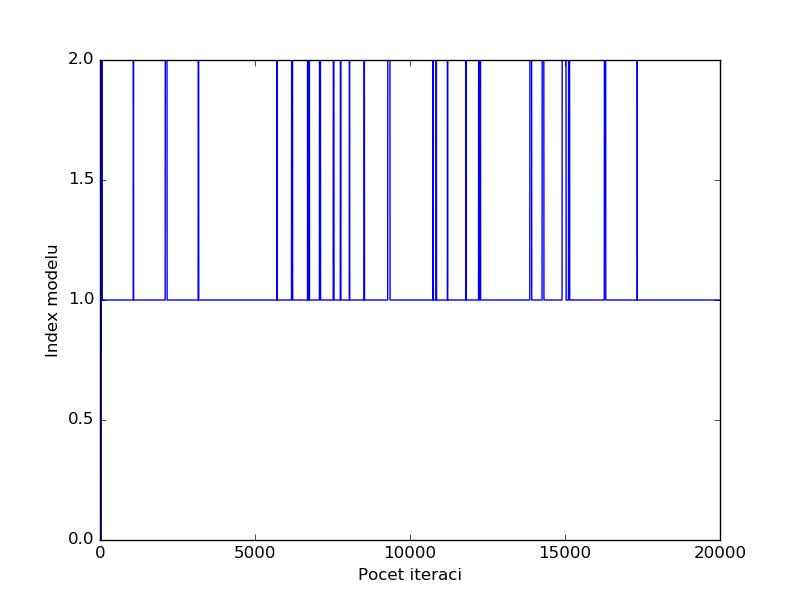
\includegraphics[width=0.8\textwidth]{images/ks_example_V.png}\caption{Vykreslení přeskoku mezi dimenzemi}\label{priklad1_prechody}
\end{figure} \par
Z vykreslení přeskoků mezi dimenzemi \ref{priklad1_prechody} je patrné, že algoritmus zůstává v modelu beze zlomu (index 0), prakticky jen nezbytně dlouho dobu než dostane možnost přeskočit do jiné dimenze a poté se už do modelu beze zlomu nikdy nevrací. Poté sice přeskakuje mezi modelem s jedním a dvěma zlomy, ale většinu času stráví v modelu s jedním zlomem. Celkově algoritmus získal 39 vzorků v modelu beze zlomu, 19233 v modelu s jedním zlomem a 728 vzorků v modelu s dvěma zlomy.
\begin{figure}
	[h]\centering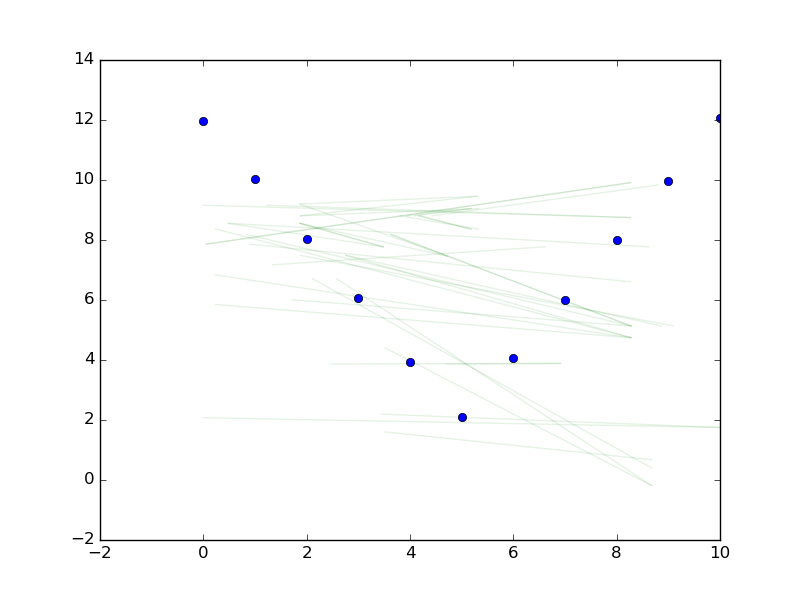
\includegraphics[width=0.8\textwidth]{images/distribution_lines_v_0breaks.png}\caption{Aproximace distribuce modelu beze zlomu}\label{v0break}
\end{figure}
\begin{figure}
	[H]\centering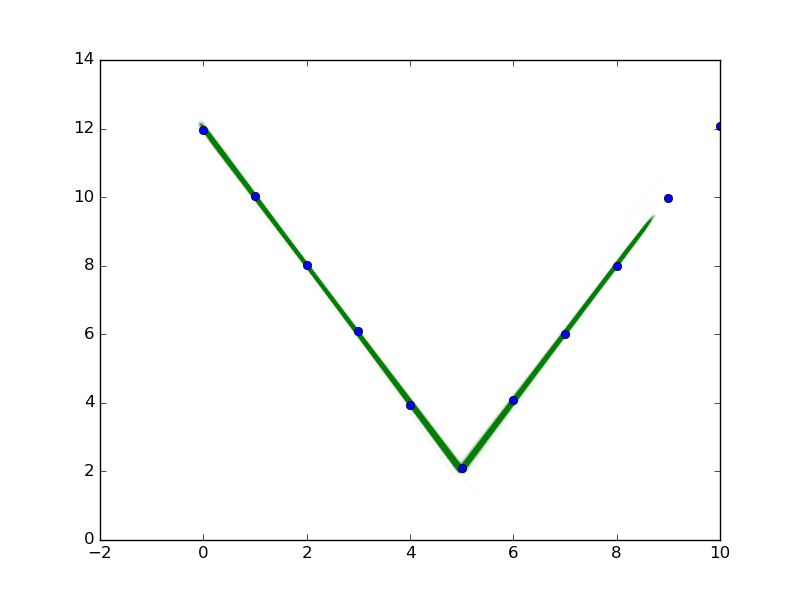
\includegraphics[width=0.8\textwidth]{images/distribution_lines_V_1break.png}\caption{Aproximace distribuce modelu s jedním zlomem}\label{v1break}
\end{figure}
\begin{figure}
	[H]\centering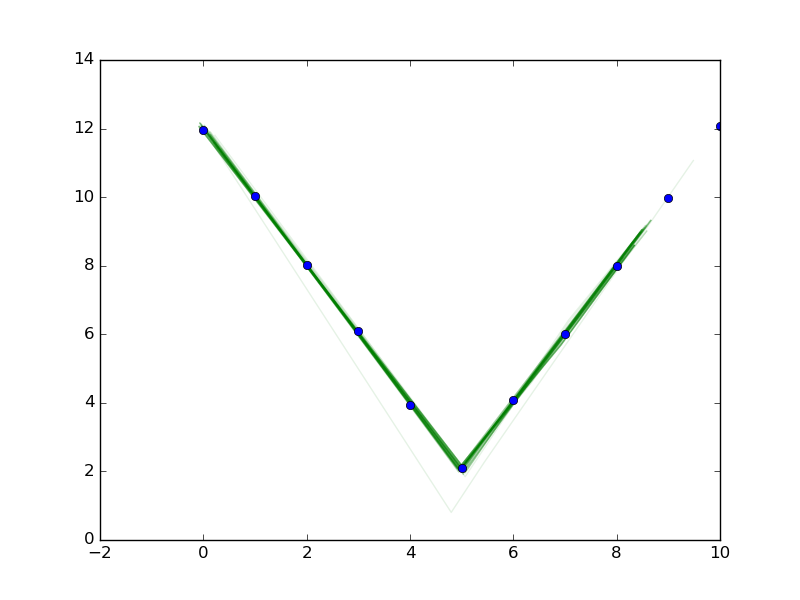
\includegraphics[width=0.8\textwidth]{images/distribution_lines_V_2breaks.png}\caption{Aproximace distribuce modelu s dvěma zlomy}\label{v2break}
\end{figure} \par
Na obrázcích \ref{v0break}, \ref{v1break}, \ref{v2break} můžeme vidět aproximace distribucí pro dané modely, pomocí vzorků z jednotlivých modelů. Zajímavé je si všimnou, faktu, že i když distribuce pro model s jedním respektive dvěma zlomy vypadají podobně, tak algoritmus strávil mnohem víc času v modelu s jedním zlomem. Je to právě dáno bayesovským přístupem, který zvýhodňuje jednodušší modely se stejnou vysvětlovací schopností. \par
Ukážeme si ještě jeden příklad a to se stejnými $x = (0, 1, 2, 3, 4, 5, 6, 7, 8, 9, 10)$ jako minule, ale $y = (20 + e_1, 15 + e_2, 7 + e_3, 1 + e_4, 1 + e_5, 1 + e_6, 1 + e_7, 11 e_8, 18 + e_9 ,25 + e_10, 32 + e_11)$ a $e_i \sim \mathcal{N}(0, 0.1)$ respektive $e_i \sim \mathcal{N}(0, 2)$. \par
V prvním případě algoritmus prakticky okamžitě přechází do modelu s dvěma zlomy a už z něj nevychází, počet vzorků v modelu 0 je 65, modelu 1 78, modelu 2 19857. V případě s vyšší dimenzí je rozdíl a to, že o hodně častěji algoritmus přechází do modelu 1. Počet vzorků v modelu 0 je 38, modelu 1 4039, modelu 2 15923. Na obrázku \ref{priklad2_prechody} je vidět jak algoritmus přechazí mezi jednotlivými modely.
\begin{figure}
	[H]\centering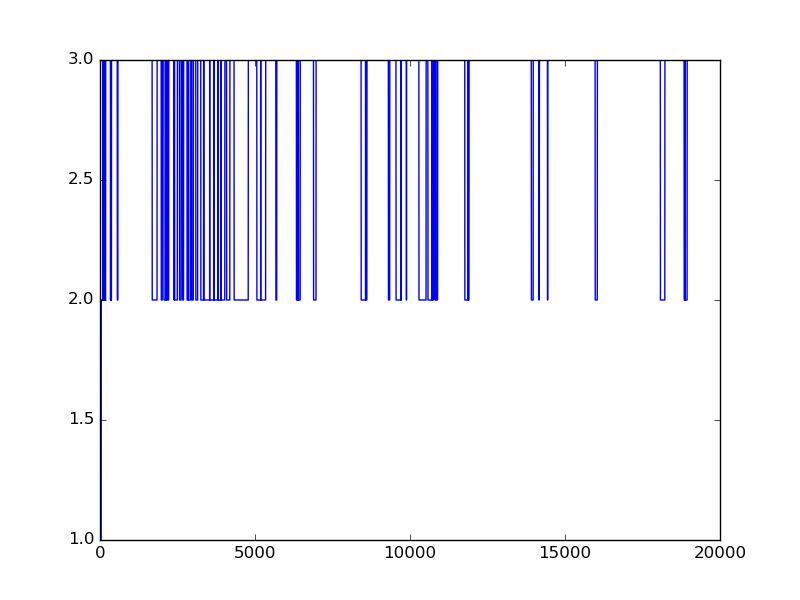
\includegraphics[width=0.8\textwidth]{images/ks_examle_u_bigger_variance.png}\caption{Vykreslení přeskoku mezi dimenzemi příklad 2, $\sigma^2 = 2$}\label{priklad2_prechody}
\end{figure}
\begin{figure}
	[H]\centering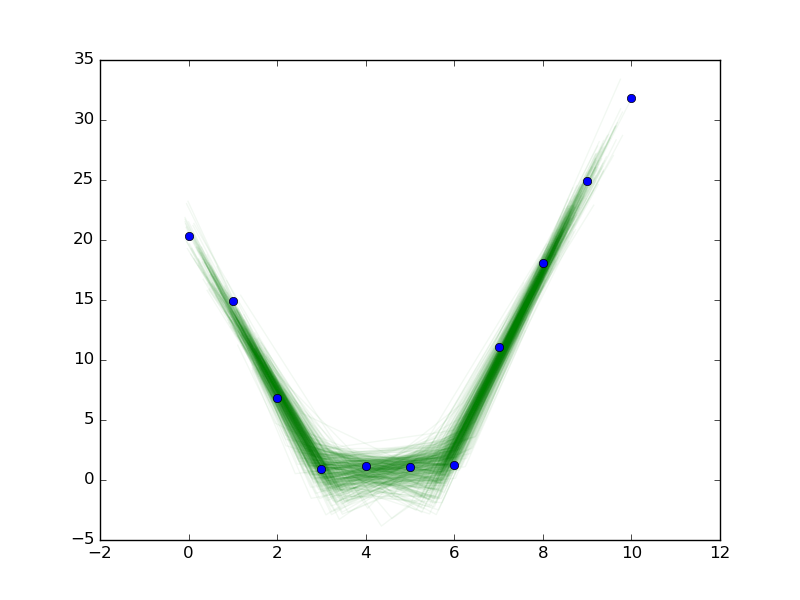
\includegraphics[width=0.8\textwidth]{images/distribution_lines_u_2breaks_small_variance.png}\caption{Aproximace distribuce modelu s dvěma zlomy, $\sigma^2 = 0.1$}\label{priklad2_distribuce_small_sigma}
\end{figure}
\begin{figure}
	[H]\centering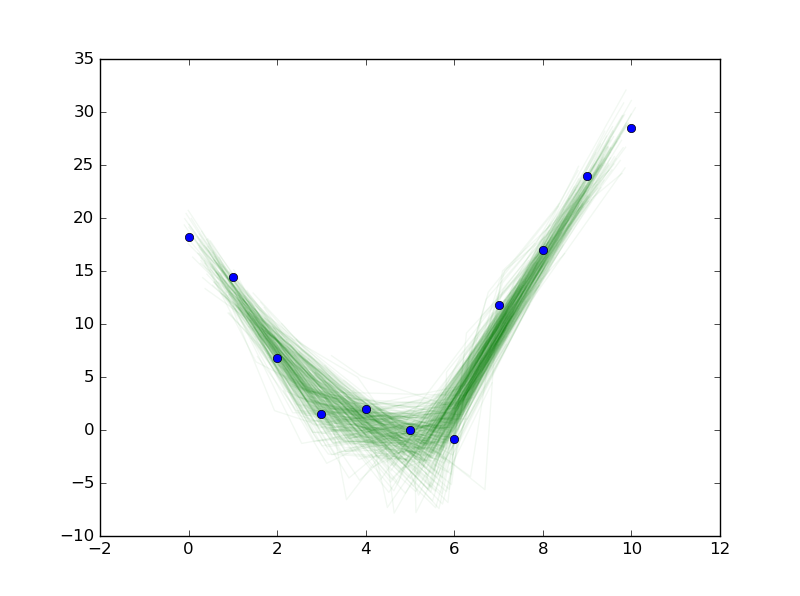
\includegraphics[width=0.8\textwidth]{images/distribution_lines_u_2breaks_bigger_variance.png}\caption{Aproximace distribuce modelu s dvěma zlomy, $\sigma^2 = 2$}\label{priklad2_distribuce_big_sigma}
\end{figure}
Na obrázcích \ref{priklad2_distribuce_small_sigma}, \ref{priklad2_distribuce_big_sigma} je vidět distribuce s menším respektive větším rozptylem. Na distribuci s menším rozptylem je vidět, že mnohem více koncentrována kolem skutečných bodů zlomu, což jsou body 3 a 6. A naopak distribuce s větším rozptylem není tak moc koncentrovaná, jak se dalo čekat.
\section{Závěr}
V práci jsme stručně popsali problémy, které se pojí s řešením po částech lineární regrese. Začli jsme úvodem do Bayesovské statistiky. V jejímž rámci jsme poté zavedli model pro po částech lineární regresi. Následně jsme si ukázali jak fungují MCMC algoritmy, které ale samy o sobě nejsou dostačující pro dosažení závěrů o našem modelu, proto jsme přešli k algoritmu RJMCMC. Ten dokáže aproximovat aposteriorní rozdělení u modelů, kde jeden z parametrů je počet ostatních parametrů. Stručně jsme popsali to jak algoritmus RJMCMC, řeší problém s přechodem mezi dimenzemi a ukázali jsme jak by takové přechody mohly vypadat. \par
Značná část naší práce spočívá v samotné implementaci algoritmu RJMCMC. Ten jsme naprogramovali v jazyce Python za pomocí knihoven NumPy a SciPy, které se používají obecně k vědeckým výpočtům a v našem případě konkrétně jsme je použili pro simulaci dat z různých pravděpodobnostních rozdělení. Také jsme použili knihovnu Theano, která slouží k symbolickým výpočtům derivací a v našem případě Jakobiánu. Na závěr naší práce jsme předvedli funkčnost naší implementace algoritmu na simulovaných datech a popsali výsledky. \par
Protože jsme přesvědčení, že naše implementace algoritmu RJMCMC je dosti obecná, přirozeným pokračováním naší práce by bylo vyzkoušení daného algoritmu na jiných problémech, jako například rozpoznávaní obrazů nebo pro směsi normálních rozdělení. Dále by si tato práce zasloužila rozvést teoretickou stránku fungování algoritmu. Protože většina reálných problému nezávisí jen na jedné veličině, bylo by dalším zajímavým rozšířením pokusit se implementovat algoritmus RJMCMC pro více dimenzionální lineární regresi. Toto by už by mohlo být značně náročné z hlediska návrhu návrhových distribucí. 

\bibliographystyle{plain}
\bibliography{bibliography}

\appendix
\section{Zdrojové kódy}
\begin{lstlisting}[caption=RJMCMC]
class Rjmcmc:
'''
trida ktera zastitute cely reversible jump markov chain
monte carlo algoritmus
'''

	def __init__(self, moves, mcmcs, stationary):
		self.moves = moves
		self.mcmcs = mcmcs
		self.stationary = stationary
		self.trans_steps = 0
		self.norm_steps = 0

	def step(self, previous_sample):
		k, theta = previous_sample
		u = uniform()
		moves = [m for m in self.moves if m.can_move(k) > 0]
		trans_probability = 0
		for m in moves:
			trans_probability += m.probability_of_this_move(previous_sample)
		if u < trans_probability:
			self.trans_steps += 1
			uu = uniform(0, trans_probability)
			M = None
			prob = 0
			for m in moves:
				if prob < uu < prob + m.probability_of_this_move(previous_sample):
					M = m
					break
				prob += m.probability_of_this_move(previous_sample)

			up, down, a, new = self.trans_step(M, previous_sample)
			return new
		else:
			self.norm_steps += 1
			if k*2 + 3 is not len(theta):
				print(k)
				print(previous_sample)
				raise AssertionError
			return (k, self.mcmcs[k].step(theta))

	def trans_step(self, move, previous_sample):
		(k, theta) = previous_sample

		new_sample, u, newu, det_jacobian = move.transform(previous_sample)

		up = np.prod([self.stationary(new_sample),
		move.probability_of_this_move(new_sample),
		move.probability_of_help_rvs(new_sample, newu)])
		down = np.prod([self.stationary(previous_sample),
		move.probability_of_this_move(previous_sample),
		move.probability_of_help_rvs(previous_sample, u)])

		a = det_jacobian*up/down
		u = uniform()

		if u < a:
			return (up, down, a, new_sample)
		else:
			return (up, down, a, previous_sample)
\end{lstlisting}
\newpage
\begin{lstlisting}[caption=implementace aposteriorního rozdělení pro po částech lineární regresi]
class Blr2:
    '''
    Trida, ktera vytvori stacionarni distribuci pro regresi s n zlomy.
    2 protoze pouzivam jinou parametrizaci.
    sigma = x[0] - rozptyl no :D
    s0 = x[1] - xova souradnice prvniho zlomu
    h0 = x[2] - yova souradnice prvnhio zlomu
    ...
    sn = x[n-2] - xova souradnice nteho zlomu
    hn = x[n-1] - yova souradnice nhteo zlomu
    '''

    def __init__(self, xs, ys, n_breaks):
        '''
        @param xs - xove souradnice dat
        @param ys - yove souradnice dat
        @param n_breaks - pocet zlomu
        '''
        if len(xs) is not len(ys):
            raise RuntimeError("Not matchin dimension")
        self.xs = xs
        self.ys = ys
        self.max_x = max(xs)
        self.min_x = min(xs)
        self.n = 2*n_breaks + 5
        self.n_samples = len(xs)
        self.h_prior = normal(np.zeros(int((self.n-1)/2)),
                              100*np.eye(int((self.n-1)/2)))
        self.sigma_prior = normal(0, 3)
        self.n_breaks = n_breaks
        
    def prior_s(self, theta):
        '''
        Apriorni rozdeleni na thetaovych souradnicich. Tedy melo by platit
        ss < s1 < s2 < ... < sn < sf. Je to tak nastaveno z toho duvodu,
        aby bylo dodrzeni poradi
        '''
        # taky si nejsem jisty jestli prochazim vsechny
        x_coordinates = [theta[i] for i in range(1, self.n, 2)]
        previous = x_coordinates[0]
        for i in range(1, len(x_coordinates)):
            if previous > x_coordinates[i]:
                return 0
            previous = x_coordinates[i]

        if x_coordinates[0] < self.min_x - 0.1:
            return 0
        if x_coordinates[len(x_coordinates) - 1] > self.max_x + 0.1:
            return 0
        return 1

    def prior_h(self, theta):
        '''
        Apriorni rozdeleni na yovych souradnicich. Je teda co nejvic
        neinformativni, tedy pro vsechny h plati, ze h ~ N(0, 100)
        '''
        # tady se trochu bojim ze neprojdu vsechny
        # jestli se dostanu za hranici tak se to rychle odhali :D
        y_coordinates = [theta[i] for i in range(2, self.n, 2)]
        return self.h_prior.pdf(y_coordinates)

    def prior_sigma(self, theta):
        '''
        Apriorni rozdeleni na rozptylu. Zas jen nake neinformativni a s
        nulovou pravdepodobnosti na sigmach mensi nez 0
        '''
        if theta[0] > 0:
            return self.sigma_prior.pdf(theta[0])
        return 0

    def likelihood(self, theta):
        '''
        Spocita likelihood hustotu pro dany vzorek
        '''
        assert len(theta) == self.n

        suma = 0
        for i, xi in enumerate(self.xs):
            yi = self.ys[i]
            for j in range(1, self.n-2, 2):
                break1 = (theta[j], theta[j+1])
                break2 = (theta[j+2], theta[j+3])

                if break1[0] <= xi < break2[0]:
                    suma += self.prob_sum(xi, yi, break1, break2)

            # tohle je pro pripad ze xi je pred nebo za body urcujicimi primku
            # stava se to :D
            if xi < theta[1]:
                break1 = (theta[1], theta[2])
                break2 = (theta[3], theta[4])
                suma += self.prob_sum(xi, yi, break1, break2)

            if xi > theta[self.n - 2]:
                break1 = (theta[self.n-4], theta[self.n-3])
                break2 = (theta[self.n-2], theta[self.n-1])
                suma += self.prob_sum(xi, yi, break1, break2)

        try:
            exp = np.exp(-suma/(2*theta[0]))
            bs = theta[0]**(-len(self.xs)/2)
            return bs * exp
        except FloatingPointError:
            print()
            print('theta0 ' + str(theta[0]))
            print('suma ' + str(suma))
            return 0

    def prob_sum(self, x, y, break1, break2):
        '''
        pomocna funkce, co mi spocita jeden vyraz v exponenciale, jakoze v
        Normalnim rozdeleni hore
        '''

        # a = (break2[1] - break1[1])/(break2[0]-break1[0])
        # b = break2[1] - break2[0]*a
        x1, y1 = break1
        x2, y2 = break2
        est = (x - x1)*(y2 - y1)/(x2 - x1) + y1
        return (y - est)**2

    def pdf(self, theta):
        if len(theta) is not self.n:
            print(theta)
            raise Exception("Co to kurva")

        prior_probs = np.prod([self.prior_h(theta),
                               self.prior_s(theta),
                               self.prior_sigma(theta)])

        # netkere vzorky budou mit nulovou pravdepodobnost
        # uz kvuli apriornimu rozdeleni, proto to checknu
        # at se nemusi pocitat likelihood ten v zavislosti
        # na datech muze byt dost narocny spocitat
        if prior_probs == 0:
            return 0
        return np.prod([prior_probs,
                        self.likelihood(theta)])

    def generate_first_sample(self):
        '''
        vygeneruje nejaky vzorek, ktery nema pravdepodobnost nula
        '''
        minimum = min(self.xs)
        maximum = max(self.xs)
        first_sample = np.zeros(self.n)

        first_sample[0] = 1

        for i, x in enumerate(np.linspace(minimum, maximum, (self.n-1)/2)):
            first_sample[2*i + 1] = x
            first_sample[2*i + 2] = np.random.normal(0, 3)

        if not self.pdf(first_sample) > 0:
            print("First sample: " + str(first_sample) +
                  " has zero probability")
            print("prior h " + str(self.prior_h(first_sample)))
            print("prior s " + str(self.prior_s(first_sample)))
            print("prior sigma " + str(self.prior_sigma(first_sample)))
            print("likelihood " + str(self.likelihood(first_sample)))
            return self.generate_first_sample()

        return first_sample
\end{lstlisting}
\newpage
\begin{lstlisting}[caption=implementace mcmc algoritmu]
class Mcmc:
    def __init__(self, proposalDistribution, stationaryDistribution):
        self.proposal = proposalDistribution
        self.stationary = stationaryDistribution

    def step(self, previous_sample):
        '''
        Vnitrek mcmc algoritmu, prakticky to co se deje v jedne 
        iteraci tady te verze hastingse
        '''
        proposal_sample = self.proposal.rvs(previous_sample)
        assert proposal_sample is not None
        local_previous_sample = copy.copy(previous_sample)
        final_sample = copy.copy(previous_sample)

        for j, x in enumerate(proposal_sample):
            local_previous_sample[j] = x
            down = np.prod([
                self.stationary.pdf(previous_sample),
                self.proposal.pdf(local_previous_sample, previous_sample)])
            up = np.prod([
                self.stationary.pdf(local_previous_sample),
                self.proposal.pdf(previous_sample, local_previous_sample)])

            u = np.random.uniform()

            if u < up/down:
                final_sample[j] = x
            else:
                local_previous_sample[j] = previous_sample[j]

        return final_sample

    def sample(self, n, first_sample):
        dimension = len(first_sample)
        samples = np.empty((n, dimension))
        samples[0] = first_sample
        # mozna generator?
        for i in range(1, n):
            samples[i] = self.step(samples[i-1])
            # progress bar
            sys.stdout.write("\r\t%.0f%% Done" % (100*i/n))
            sys.stdout.flush()
        # progress konec
        sys.stdout.write("\r\t100% Done\n")
        sys.stdout.flush()
        return samples
\end{lstlisting}
\newpage
\begin{lstlisting}[caption=Implementace přeskoků mezi dimenzemi]
class Move:
    '''
    predstavuje prechod z k do k' a zpet
    '''

    def __init__(self,
                 k1,
                 k2,
                 k1_to_k2,
                 k2_to_k1,
                 transform1to2,
                 transform2to1,
                 jacobian1to2,
                 jacobian2to1,
                 ugenerator1to2,
                 ugenerator2to1,
                 usize1,
                 usize2):
        '''
        k1 - prvni stav
        k2 - druhy stav
        k1_to_k2 - pravdepodobnost prechodu z k1 do k2
        k2_to_k1 - pravdepodobnost prechodu z k2 do k1
        transform1to2 - pretransformuje vzorek na vzorek s jinou dimenzi
                        vraci novy vzorek a mozne nahodne cisla, ktere
                        by byly vegenerovane pro zpetnou transformaci
        transform2to1 - ---||---
        ugenerator1to2 - generator pomocnych nahodnych velicin pro prechod
                         z k1 do k2
        ugenerator2to1 - ---||---
        usize1 - delka vektoru nahodnych velicin ktery se vygeneruje pro prechod ze 
                 stavu 1 do stavu 2
        usize2 - ---||---
        '''
        self.k1 = k1
        self.k2 = k2
        self.k1_to_k2 = k1_to_k2
        self.k2_to_k1 = k2_to_k1
        self.transform1to2 = transform1to2
        self.transform2to1 = transform2to1
        self.jacobian1to2 = jacobian1to2
        self.jacobian2to1 = jacobian2to1
        self.ugenerator1to2 = ugenerator1to2
        self.ugenerator2to1 = ugenerator2to1
        self.usize1 = usize1
        self.usize2 = usize2

    def can_move(self, k):
        '''
        urci jestli muzu pouzit tento prechod z daneho stavu
        '''
        if k == self.k1:
            return self.k1_to_k2
        elif k == self.k2:
            return self.k2_to_k1
        else:
            return 0

    def probability_of_this_move(self, x):
        '''
        pravdepodobnost pouziti tohole typu pohybu z daneho
        stavu. zatim pouzivame jen dany stav k, ale v algoritmu
        je mozne i pouzit pro vypocet pravdepodobnosti soucasny
        vzorek. takze ted ty prechodove pravdepodobnosti jsou jenom
        konstanty, ale obecne by to mohla byt i funkce
        '''
        k, theta = x
        if self.k1 == k:
            return self.k1_to_k2
        elif self.k2 == k:
            return self.k2_to_k1
        else:
            raise RuntimeError("This should never happen")

    def _transform(self, k, newk, theta, generator, transform, newu_size):
        if generator is not None:
            u = generator.rvs()
            ext_theta = np.append(theta, u)
        else:
            u = None
            ext_theta = theta
        newtheta = transform(ext_theta)

        if newu_size is not 0:
            newu = newtheta[-newu_size:]
            newtheta = newtheta[:-newu_size]
        else:
            newu = None
        newx = (newk, newtheta)
        det_jacobian = self.get_jacobian((k, ext_theta))
        return (newx, u, newu, det_jacobian)

    def transform(self, x):
        # tady by se rovnou mohl vracet i ten jacobian at se s tim neseru venku
        k, theta = x
        if self.k1 == k:
            return self._transform(k,
                                   self.k2,
                                   theta,
                                   self.ugenerator1to2,
                                   self.transform1to2,
                                   self.usize2)
        elif self.k2 == k:
            return self._transform(k,
                                   self.k1,
                                   theta,
                                   self.ugenerator2to1,
                                   self.transform2to1,
                                   self.usize1)
        else:
            raise RuntimeError("This shoould never happen")

    def probability_of_help_rvs(self, x, u):
        k, theta = x
        if self.k1 == k:
            if self.ugenerator1to2 is None:
                return 1
            return self.ugenerator1to2.pdf(u)
        elif self.k2 == k:
            if self.ugenerator2to1 is None:
                return 1
            return self.ugenerator2to1.pdf(u)
        else:
            raise RuntimeError("This should never happen")

    def get_jacobian(self, x):
        k, theta = x
        if self.k1 == k:
            mat = self.jacobian1to2(theta)
            return np.linalg.det(mat)
        elif self.k2 == k:
            mat = self.jacobian2to1(theta)
            return np.linalg.det(mat)
        else:
            raise RuntimeError("This should never happen")
\end{lstlisting}
\end{document}

 
